\documentclass[informe.tex]{subfiles}
\begin{document}

Los filtros digitales que son realizables mediante elementos computacionales estarán dados por una función racional en $z^{-1}$

	$$
		H(z)= \frac{ \sum_{ k=0 }^{ M }{ b_k z^{-k}} }
		           { 1 - \sum_{ k=1 }^{ N }{ b_k z^{-k}} }
		= \frac{Y(z)}{X(z)}
	$$
o de forma equivalente

	$$
		Y(z)=\sum_{k=1}^{N}{a_k Y(z) \cdot z^{-k}} + \sum_{k=0}^{M}{b_k X(z) \cdot z^{-k}}
	$$

y en la caracterización correspondiente en tiempo discreto estará dada por una ecuación de diferencias.

	\begin{equation}
		\label{eqn:ec:dif}	
		y(n)=\sum_{k=1}^{N}{a_k y(n-k)} + 
		            \sum_{k=0}^{M}{b_k x(n-k)}
	\end{equation}
	
La realización del filtro digital se expresa mediante un algoritmo, que puede a su vez puede ser construido en hardware dedicado o hardware de propósito general mediante software. En ambos casos, realizados a través de elementos computacionales sencillos, tales como, sumas (Fig. \ref{fig:realizacion:suma}), productos de constantes (Fig. \ref{fig:realizacion:multiplicacion}), y retardos temporales (Fig. \ref{fig:realizacion:retardo}).\newline
 
\begin{figure}[h]
     \centering
     \begin{subfigure}[b]{0.3\textwidth}
         \centering
         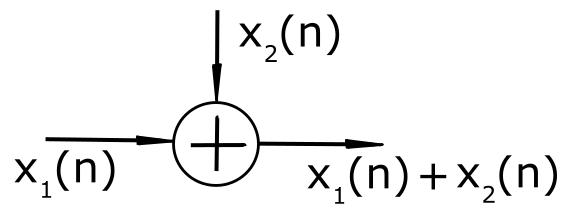
\includegraphics[scale=0.2]{realizacion_suma.jpg}
         \caption{Suma de señales}
         \label{fig:realizacion:suma}
     \end{subfigure}
     \hfill
     \begin{subfigure}[b]{0.3\textwidth}
         \centering
         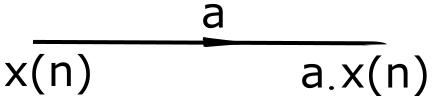
\includegraphics[scale=0.2]{realizacion_multiplicacion.jpg}
         \caption{Multiplicación de señal por constante}
         \label{fig:realizacion:multiplicacion}
     \end{subfigure}
     \hfill
     \begin{subfigure}[b]{0.3\textwidth}
         \centering
         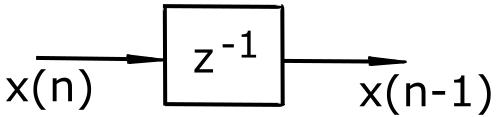
\includegraphics[scale=0.2]{realizacion_retardo.jpg}
         \caption{Retardo unitario}
         \label{fig:realizacion:retardo}
     \end{subfigure}
 		\caption{Representación en bloques de elementos computacionales básicos}
        \label{fig:realizacion:elementos_computacionales}
\end{figure}

Estos algoritmos se dan en diferentes estructuras o tipologías que representan en diagramas de bloques, diagramas de flujo o notación matricial. Entre estas estructuras se encuentran:\newline

1- Formas directas: la $H(z)$ se realiza en una sola pieza. Se clasifican en Formas directas I y II, estructura de escalera, estructura de celosías, extracción de multiplicadores, y formas modulares de filtros de ondas.\newline

2- Formas indirectas: la $H(z)$ se descompone en varias secciones de primer y segundo orden.  Mediante las formas directas se consiguen estructuras de primer y segundo orden, y luego se combinan de algún modo, como en cascada.\\\\

\textbf{Forma directa I y II}\\

La Ec. \ref{eqn:ec:dif} puede ser representada por el diagrama de bloques como muestra la Fig. \ref{fig:realizacion:diagrama} y puede ser reorganizado con el diagrama de la Fig. \ref{fig:realizacion:forma_directa_I}, esta última forma se denomina forma directa I. 

	\begin{figure}[h]
		\centering
		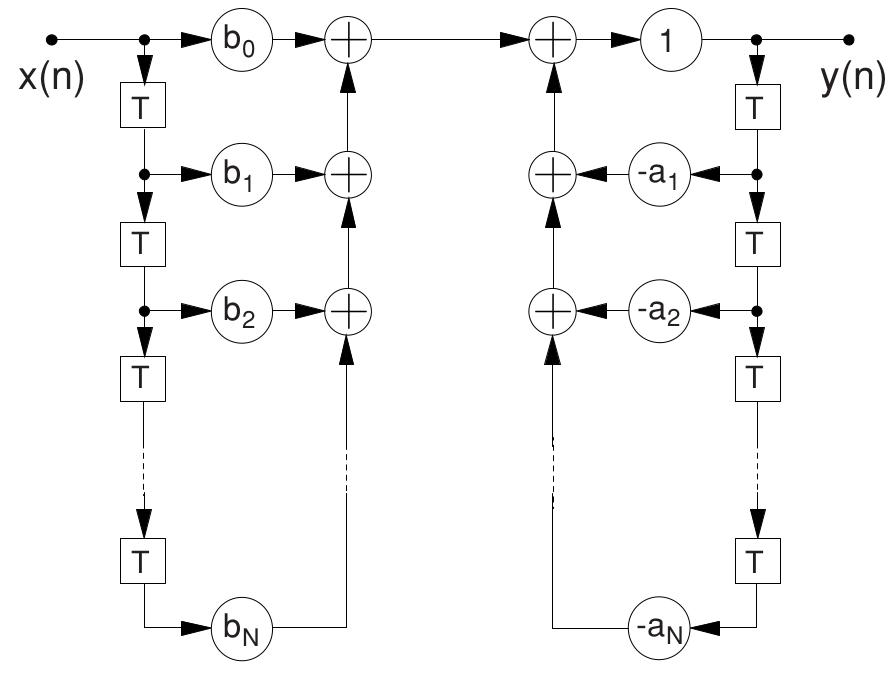
\includegraphics[scale=0.4]{realizacion_diagrama_de_bloque.jpg}	
		\caption{Representación de la Ec. \ref{eqn:ec:dif} }
		\label{fig:realizacion:diagrama}
	\end{figure}	

El flujo de las señales que se dirigen hacia los bloques de retardo que representa la forma directa I se pueden cambiar de tal forma que permitan reorganizar los bloques combinando dos retardos en un solo bloque. Esto permitiría ahorrar unidades de memoria al minimizar los registros de desplazamiento paralelos utilizados para realizar para realizar los retardos, esta forma se denomina segunda forma canónica o forma directa II y se muestra en la Fig. \ref{fig:realizacion:forma_directa_I}.

\begin{figure}[h]
	\centering
	\begin{subfigure}[b]{0.4\textwidth}
	\centering
		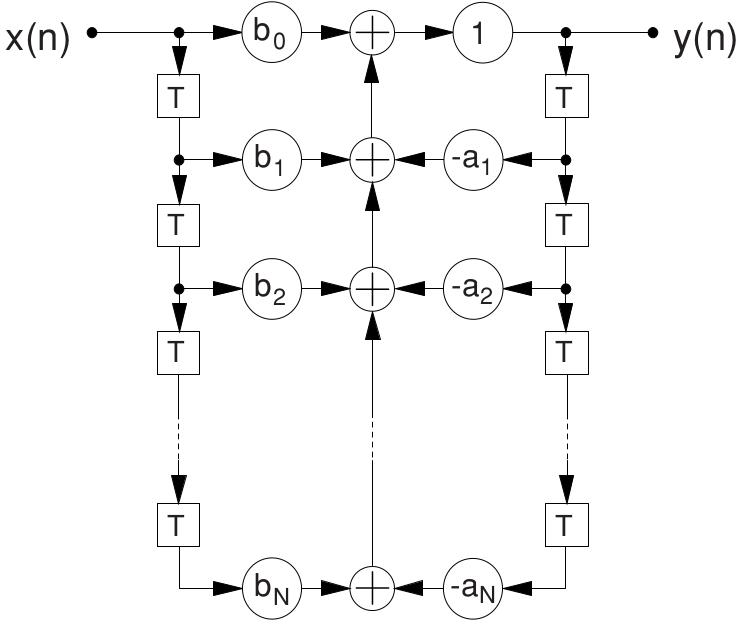
\includegraphics[scale=0.4]{realizacion_forma_ditecta_I.jpg}
		\caption{Forma directa I}
		\label{fig:realizacion:forma_directa_I}
	\end{subfigure}
	\bigskip
	\begin{subfigure}[b]{0.4\textwidth}
		\centering
		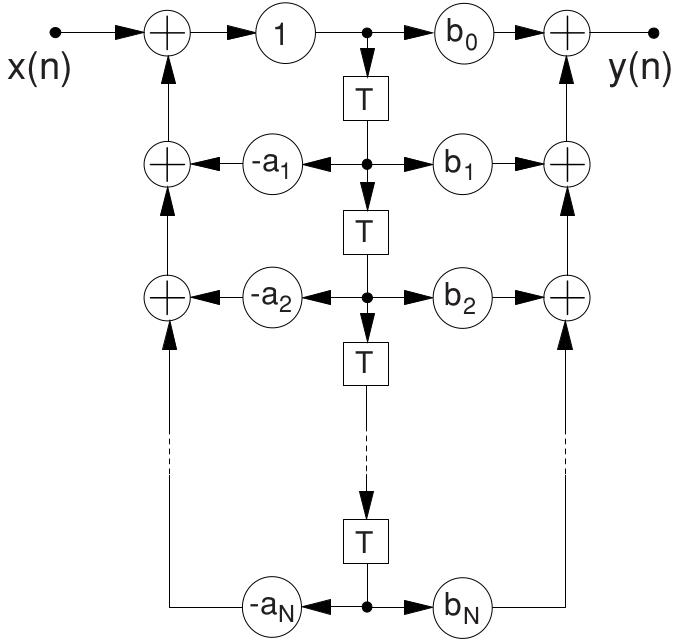
\includegraphics[scale=0.4]{realizacion_forma_ditecta_II.jpg}
		\caption{Forma directa II}
		\label{fig:realizacion:forma_directa_I}
	\end{subfigure}  
	\caption{Forma directa I y II}
	\label{fig:realizacion:forma_directa}
\end{figure}

\end{document}	